\section{Desarrollo Basado en Pruebas y Comportamientos} \label{sect:TDD_BDD}

El proceso descrito por la metodología \textit{Scrum} no establece prácticas especificas para la construcción del producto. Es por esto que en Empresas TD se integran los principios del desarrollo Basado en Pruebas o \textit{Test Driven Development} (TDD)  y el Desarrollo Basado en Comportamientos, en inglés \textit{Behavior Driven Development} (BDD), como practicas a seguir durante el fase de programación. El procedimiento de desarrollo usando TDD se muestra en la figura \ref{img:tdd}.

\begin{figure}[h]
	\begin{center}
		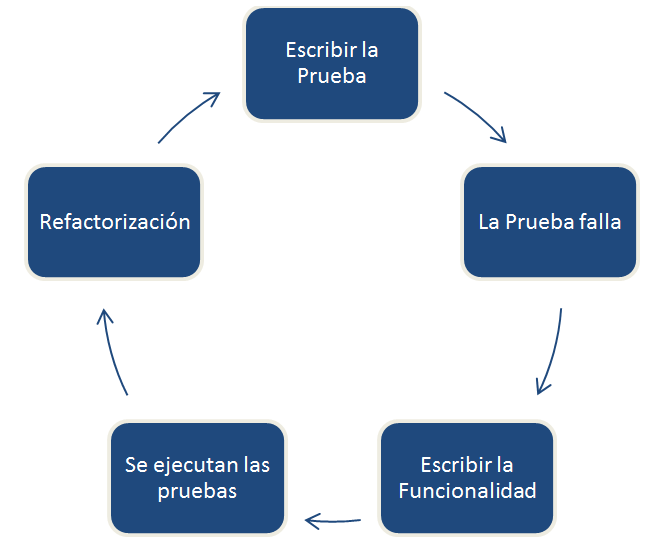
\includegraphics[scale=0.55]{imagenes/tdd.png}
	\end{center}
	\caption{
		\label{img:tdd}
		Ciclo de \textit{Test Driven Development}
	}
\end{figure}

En primer lugar, se escribe una prueba y se verifica que ésta falla. Luego se implementa el código que hace que la prueba pase satisfactoriamente y seguidamente se refactoriza el código escrito. Por último, se agrega una nueva prueba y se inicia el proceso nuevamente. Esta técnica es utilizada hasta que la funcionalidad deseada este completa y trabaja adecuadamente. 

La forma más efectiva de aplicar esta técnica es segmentar la funcionalidad en pequeñas unidades que puedan ser probadas de manera automatizada e inequívoca, así se genera código simple y fácil de mantener gracias al proceso de refactorización asociado. Sin embargo aplicar esta técnica por sí sola es complejo, puesto que en ocasiones es difícil determinar qué probar y en qué nivel de detalle.

BDD surge como una manera de subsanar esta dificultad. En lugar de basar las pruebas en pequeñas unidades de funcionalidad, BDD establece que las pruebas deben reflejar los comportamientos deseados por los diferentes actores involucrados en el proyecto. 

Para que se pueda aplicar BDD de manera adecuada es de vital importancia que todos los involucrados manejen un mismo léxico con respecto al proyecto, que les permita describir los comportamientos deseados en términos comunes sin caer en detalles de implementación. BDD sugiere la utilización de un esquema similar al siguiente para especificar los comportamientos \cite{IBDD}.

\begin{itemize}
\item Dado: Un contexto inicial.
\item Cuando: El evento a probar ocurre.
\item Entonces: Se aseguran que se alcancen los resultados deseados.
\end{itemize}

Este enfoque permite que las especificaciones no deban ser reescritas ya que el comportamiento pocas veces cambia durante el desarrollo, sólo cambia la implementación. Además facilita el proceso de determinar los requerimientos mientras que acelera la documentación.



 

